\documentclass[tikz]{standalone}
\usepackage{pgfplots}
\usepackage{xcolor}
\usetikzlibrary{calc}
\definecolor{mycolor}{HTML}{ffd966}
\pgfplotsset{compat=1.18}

\begin{document}
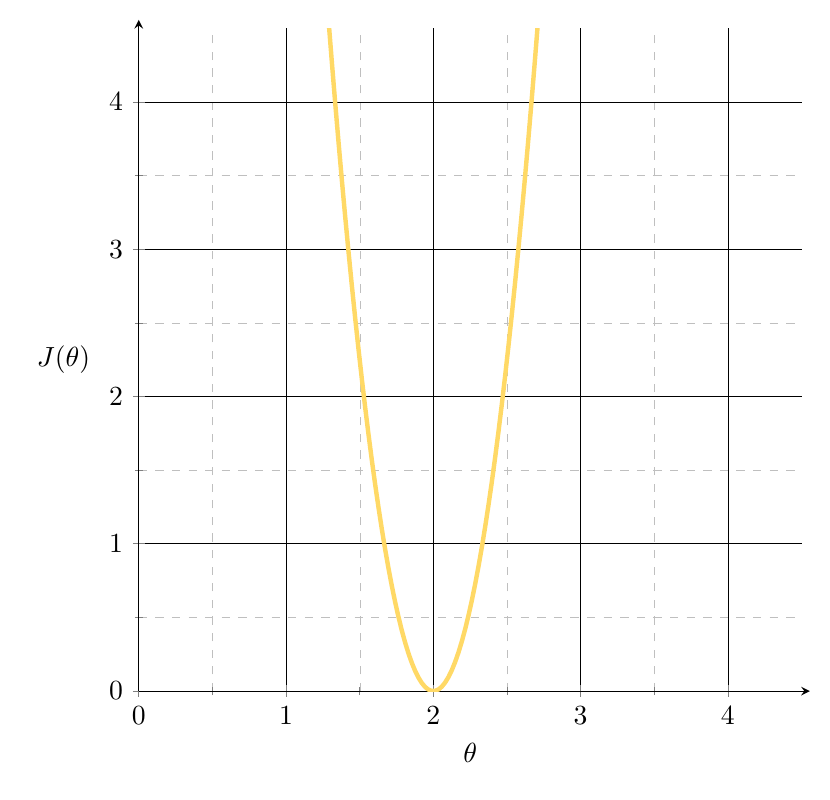
\begin{tikzpicture}
  \begin{axis}[
    axis lines=left,
    x axis line style={->,>=stealth, shorten >=-3pt},
    y axis line style={->,>=stealth, shorten >=-3pt},
    xlabel={\(\theta\)},
    ylabel={\(J(\theta)\)},
    ylabel style={rotate=-90},
    xmin=0, xmax=4.5,
    ymin=0, ymax=4.5,
    xtick={0,1,...,4},
    ytick={0,1,...,4},
    minor x tick num=1,
    minor y tick num=1,
    grid=both,
    major grid style={line width=0.2pt,draw=black},
    minor grid style={line width=0.1pt,draw=gray!50,dashed},
    width=10cm,
    height=10cm,
  ]
    % J(theta) = (3*theta - 6)^2 = 9*(theta - 2)^2
    % Minimum at theta* = 2, J(2) = 0
    \addplot[domain=0:4.5, samples=200, ultra thick, color=mycolor]
      {9*(x - 2)^2};
  \end{axis}
\end{tikzpicture}
\end{document}
